\documentclass[usegraphicx,usenatbib]{mn2e}

\usepackage{verbatim}
\usepackage{color}
\usepackage[normalem]{ulem} % for striking out with \sout
\usepackage{amsmath} % for boldsymbol
% A comment block

%\newcommand{\comment}[1]{}

% For color
\newcommand{\mpname}[1]{#1_color.eps}
\newcommand{\clraitoff}{red}
\newcommand{\lumblack}{(black)}
\newcommand{\lumblue}{(blue)}
\newcommand{\lumred}{(red)}
\newcommand{\vdisred}{(red-dashed curve)}
\newcommand{\vdisblue}{(blue-solid curve)}

% For bw
%\newcommand{\mpname}[1]{#1.eps}
%\newcommand{\clraitoff}{}
%\newcommand{\lumblack}{}
%\newcommand{\lumblue}{}
%\newcommand{\lumred}{}
%\newcommand{\vdisred}{(dashed curve)}
%\newcommand{\vdisblue}{(solid curve)}

\newcommand{\umag}{$u$}
\newcommand{\gmag}{$g$}
\newcommand{\rmag}{$r$}
\newcommand{\imag}{$i$}
\newcommand{\zmag}{$z$}
\newcommand{\gmr}{$g-r$}



\newcommand{\gammat}{$\gamma_T$}
\newcommand{\gammacross}{$\gamma_\times$}
\newcommand{\deltasig}{$\Delta \Sigma$}
\newcommand{\deltaplus}{$\Delta \Sigma_+$}
\newcommand{\deltacross}{$\Delta \Sigma_\times$}
\newcommand{\deltarho}{$\Delta \rho$}
\newcommand{\movr}{$M(<r)$}
\newcommand{\sigmacrit}{$\Sigma_{crit}$}

\newcommand{\photoz}{photo-z}
\newcommand{\photozs}{photo-zs}

\newcommand{\tlum}{$L^{tot}$}
\newcommand{\tngal}{$N_{gal}^{tot}$}

\newcommand{\lstarlim}{$0.4 L_*$}
\newcommand{\lvir}{$L_{200}$}
\newcommand{\nvir}{$N_{200}$}
\newcommand{\rvir}{$r_{200}^{gals}$}

\newcommand{\ngal}{$N_{gal}$}
\newcommand{\maxbcg}{maxBCG}
\newcommand{\numNgalBins}{12}
\newcommand{\numLumBins}{16}

\newcommand{\tngalAperture}{2$h^{-1}$ Mpc}

\newcommand{\photo}{\texttt{PHOTO}}
\newcommand{\astrop}{\texttt{ASTRO}}
\newcommand{\mt}{\texttt{MT}}
\newcommand{\spectro}{\texttt{SPECTRO}}
\newcommand{\spectroone}{\texttt{SPECTRO1d}}
\newcommand{\spectrotwo}{\texttt{SPECTRO2d}}
\newcommand{\target}{\texttt{TARGET}}

\newcommand{\lenszmax}{0.3}
\newcommand{\lenszmin}{0.05}

\newcommand{\photoversion}{\texttt{v5\_4}}

%\def\eone{e$_1$}
%\def\etwo{e$_2$}
\newcommand{\etan}{e$_+$}
\newcommand{\erad}{e$_\times$}
\newcommand{\eclass}{\texttt{ECLASS}}
\newcommand{\eclasscut}{-0.06}
\newcommand{\gmrcut}{0.7}

\newcommand{\hrs}{$^{\mathrm h}$}
\newcommand{\minutes}{$^{\mathrm m}$}

\newcommand{\ugriz}{$u, g, r, i, z$}
\newcommand{\polarization}{polarization}

\newcommand{\wgm}{$w_{gm}$}
\newcommand{\wgg}{$w_{gg}^p$}
\newcommand{\wmm}{$w_{mm}$}
\newcommand{\xigg}{$\xi_{gg}$}
\newcommand{\ximm}{$\xi_{mm}$}
\newcommand{\xigm}{$\xi_{gm}$}

\newcommand{\numspec}{127,001}
\newcommand{\numspecvlim}{10,277}
\newcommand{\numrand}{1,270,010}
\newcommand{\numspectot}{278,192}
\newcommand{\numvdis}{49,024}
%\newcommand{\numsource}{10,259,949}
% hirata: 
\newcommand{\nummask}{1,815,043}
\newcommand{\numTenMpc}{132,473}
\newcommand{\numThirtyMpc}{101,221}
\newcommand{\numsource}{27,912,891}

\newcommand{\numpairsTenMpc}{2,670,898,177}
\newcommand{\altnumpairsTenMpc}{2.7 billion}
\newcommand{\numpairsThirtyMpc}{14,818,082,122}
\newcommand{\altnumpairsThirtyMpc}{14.8 billion}



\newcommand{\xirmax}{$\xi_{gm}(R_{max})$}


\def\eps@scaling{1.0}% 

\newcommand{\sn}{$S/N$}
\newcommand{\Msn}{$(S/N)_{\textrm{matched}}$}
\newcommand{\Tsn}{$(S/N)_{\textrm{size}}$}
\newcommand{\fsn}{$(S/N)_{\textrm{flux}}$}

% stolen from the BA14 source
\newcommand{\vecg}{\mbox{\boldmath $g$}}
\newcommand{\vecD}{\mbox{\boldmath $D$}}
\newcommand{\vecQ}{\mbox{\boldmath $Q$}}
\newcommand{\matR}{\mbox{$\bf R$}}
\newcommand{\matC}{\mbox{$\bf C$}}
\newcommand{\bnabg}{ \boldsymbol{\nabla_g}}

\newcommand{\desreq}{$4\times 10^{-3}$}
\newcommand{\lsstreq}{$2\times 10^{-3}$}

\newcommand{\sersic}{S\'{e}rsic}

\newcommand{\lognormscatt}{30}

\newcommand{\mnras}{MNRAS}%
\newcommand{\apj}{ApJ}%
\newcommand{\aj}{AJ}%
\newcommand{\pasp}{PASP}%
\newcommand{\jcp}{J.~Chem.~Phys.}

%\slugcomment{Last revision \today}
%\shortauthors{Sheldon}
%\shorttitle{Bayesian Shear Estimation}

\begin{document}

\title{On Bayesian Shear Estimation}

\author[Erin S. Sheldon]{Erin S. Sheldon\thanks{E-mail: erin.sheldon@gmail.com}\\
Brookhaven National Laboratory, Bldg 510, Upton, New York 11973}

\maketitle

\begin{abstract}

The Bayesian gravitational shear estimation algorithm developed by \cite{ba14}
can potentially be used to overcome noise bias and recover shear using very low
signal-to-noise ratio (\sn) galaxy images.  In that work the authors confirmed
the method is sufficiently unbiased for planned surveys ($\Delta g/g < 2 \times
10^{-3}$) in a simplified demonstration, but no test was performed on images.
Here I present a full implementation for fitting models to galaxy images,
including the effects of a point spread function (PSF) and pixelization.  I
tested the implementation using simulated galaxy images modeled as \sersic\
profiles with $n=1$ (exponential) and $n=4$ (\devauc), convolved with a PSF and
a flat pixel response function.  I used a round Gaussian model for the PSF to
avoid potential PSF-fitting errors. I simulated galaxies with mean {\it
observed, post-PSF} full-width at half maximum equal to approximately 1.2 times
that of the PSF, with log-normal scatter.  I generated fluxes with
log-normal scatter and a discrete set of mean fluxes tuned to produce various
optimal, matched signal-to-noise ratios in the range $10-1000$.  I applied a
constant shear to all images. I fit the simulated images to a model with the
true \sersic\ index to avoid modeling biases.   Under these controlled
conditions I recovered the input shear with fractional error $\Delta g/g < 2
\times 10^{-3}$ in all cases, confirming the method is sufficiently unbiased
for planned surveys.  This demonstration can be considered a
proof-of-principle, and encouragement for the implementation of a
model-independent approach.


\end{abstract}

\section{Introduction} \label{sec:intro}


Noise bias is one of the largest potential systematic errors in weak
gravitational shear measurements.  Noise bias is a multiplicative calibration
error, associated with some point estimators for shear in the presence of
noise, such as a maximum likelihood estimate or expectation value for the
ellipticity of a galaxy \citep{HirataAlign04,Refreg12,Melchior12,Miller13}.
Averaging these point estimators gives a biased estimate of the shear.  The
bias remains even when response terms are included, such as that introduced by
\cite{ksb95} and \cite{Bern02}. It may be possible to derive point estimators
for the shear for which the average is unbiased, even in the presence of large
noise, but no such estimator currently exists.

At flux signal-to-noise ratio (\sn) $\sim 10$, the noise bias can be of order
10\% for galaxies with size comparable to that of the of the
point-spread-function (PSF).  This multiplicative error is significantly larger
than the requirements for planned and current surveys, which are $\sim$0.2\%
and $\sim$0.4\%, respectively \citep{HutererSystematics06}.

A Bayesian approach to shear estimate was proposed by \cite{Miller07}
specifically to address noise bias.  With that method, a point estimator for
the shear is still used (the expectation value of the galaxy ellipticity), but
a response term is calculated based on prior information of the true
distribution of galaxy ellipticities and the likelihood surface for a given
galaxy.  A limitation of this method is that no expression was derived for the
mean shear from an ensemble of galaxies, rather it was proposed to average the
responses from individual galaxies.  This pioneering approach performs well in
comparison to many previous methods, but does not meet the requirements for
current and planned surveys \citep{ba14}.

Other approaches have been proposed. For example \cite{Zuntz13} propose to use
a point estimate from galaxy shapes and simply calibrate the answer using
simulated data.  A related idea has been proposed in schematic form by
\cite{Refregier13}, to use an iterative approach where the universe is
simulated and its parameters tuned, along with calibration parameters of the
measurement, to reproduce the observed results.  These methods are in principle
limited only by the accuracy of the simulations to represent the real universe.

A rigorous Bayesian formalism was developed by \cite{ba14}, hereafter BA14,
that has the potential to recover shear with good accuracy using even very low
\sn\ galaxy images.  Rather than relying on a point estimate for the shear,
they derived an expression for the mean shear estimated from an ensemble of
measurements, exploiting the fact that the posterior for the shear must
approach a Gaussian for a large ensemble.  They showed that the method is
sufficiently unbiased for current and planned surveys in a simple demonstration
with galaxy ellipticities only, but no implementation for use with galaxy
images was presented.

Here I present a full model-fitting implementation of the BA14 algorithm that
works on galaxy images, including the effects of the PSF and pixelization.  I
test the implementation using a set of image simulations with idealized galaxy
models, and show that under these controlled conditions the method is
sufficiently accurate for current and planned surveys.

Below I follow the notation of BA14, where a shear was represented by the
glyph \vecg.

\section{Algorithm} \label{sec:algo}

The full algorithm is presented in BA14.  There are two important assumptions
underlying this approach (following the notation in BA14):

\begin{itemize}

    \item The shear is weak, $\vecg \ll 1$.

    \item The posterior distribution of the mean shear derived from a large
        ensemble of galaxy images is approximately Gaussian.

\end{itemize}

The assumption of small shear is true under many circumstances, but breaks down
along lines-of-sight near large over-densities, such as clusters of galaxies.

The second assumption follows from the central limit theorem: if the shear is
derived from a large enough ensemble of galaxy shapes, the posterior
necessarily approaches a Gaussian.

No information is necessarily ``lost'' by restricting shear estimation to
populations rather than individual galaxies.  The likelihood or posterior
distribution for a parameter derived from a single galaxy will not generally be
Gaussian except in the limit of high signal-to-noise ratio (\sn). Even if such
high \sn\ galaxies could be used, galaxies have intrinsic shapes that are a
large effective noise for shear measurement.  Some kind of averaging must be
performed to extract a shear from galaxy shapes.  


Under these assumptions, the authors of BA14 derived a second-order Taylor
expansion of the logarithm of the shear posterior about zero shear, consistent
with the Gaussian assumption:
%\begin{equation} \label{eq:pexpand}
%-\ln P(\vecg | \vecD) \approx {(\rm const)} 
%    - \ln P(\vecg) - \vecg \cdot \sum_i
%    \frac{\vecQ_i}{P_i}
%    + \frac{1}{2} \vecg \cdot \left[ \sum_i \left(\frac{\vecQ_i \vecQ^T_i}{P_i^2}
%    - \frac{\matR_i}{P_i}\right) \right] \cdot \vecg,
%\end{equation}
\begin{eqnarray} \label{eq:pexpand}
    -\ln P(\vecg | \vecD) & \approx & {(\rm const)} - \ln P(\vecg) \nonumber \\
                          & & - \vecg \cdot \sum_i \frac{\vecQ_i}{P_i} \\
    & &
    + \frac{1}{2} \vecg \cdot \left[ \sum_i \left(\frac{\vecQ_i \vecQ^T_i}{P_i^2}
    - \frac{\matR_i}{P_i}\right) \right] \cdot \vecg, \nonumber
\end{eqnarray}
where \vecD\ is the data vector and \vecg\ is the two-component shear.  The
terms $P_i$, $\vecQ_i$, and $\matR_i$ are 
\begin{eqnarray} \label{eq:pqrdef}
P_i     & = & P(\vecD_i | \vecg=0) \nonumber \\
\vecQ_i & = & \left. \bnabg P(\vecD_i | \vecg)\right|_{\vecg=0} \\
\matR_i & = & \left. \bnabg \bnabg P(\vecD_i | \vecg)\right|_{\vecg=0}. \nonumber
\end{eqnarray}
$P$ is the Bayesian ``prior'', and functionally corresponds to the true
distribution of all the relevant galaxy parameters in the absence of shear.
Note the prior on the shear $P(\vecg)$ is assumed to be uninformative, and is
treated as effectively constant in what follows.

Accurate prior information for the galaxy shapes is important for this method:
the derivatives of the un-lensed distribution of shapes with respect to shear
encode how the ensemble of galaxy images responds to a shear. With knowledge of
the true population of shapes, and how that population transforms under shear,
one can infer the applied shear, even in the presence of noise.

To predict the observed distribution of shapes in general, the un-lensed
distribution of shapes must be mathematically sheared and compared to
observables.  However in the approximation given above, only derivatives near
$g=0$ are required and the mean shear $\bar{\vecg}$ and covariance matrix
$\matC_g$ can be found directly:
\begin{eqnarray}
\matC_g^{-1} & = & \sum_i \left(\frac{\vecQ_i \vecQ^T_i}{P_i^2} - \frac{\matR_i}{P_i}\right) \label{eq:cdef} \nonumber \\
\bar{\vecg} & = &  \matC_g \sum_i \frac{\vecQ_i}{P_i}. \label{eq:shdef}
\end{eqnarray}

In practice the parameters of each galaxy are not precisely known. In that case
the derivatives in equation \ref{eq:pqrdef} can be averaged over the full
likelihood surface for each galaxy, taking care to use the prior
distribution given the shear.  These mean values can then be used in the
aggregates shown in Equation \ref{eq:shdef}.
%\begin{equation} \label{eq:marg}
%P_i     & = & P(\vecD_i | \vecg=0) \nonumber \\
%\vecQ_i & = & \left. \bnabg P(\vecD_i | \vecg)\right|_{\vecg=0} \\
%\matR_i & = & \left. \bnabg \bnabg P(\vecD_i | \vecg)\right|_{\vecg=0}. \nonumber
%\end{equation}

A conceptual outline for measurement of non-constant shear was also given by
BA14, as were third-order tweaks to the second-order perturbations.

A full implementation, fitting to pixelized galaxy images, was not attempted in
BA14.  The basic formalism was shown to work by drawn shapes randomly from an
analytic distribution, adding noise and a small shear, and recovering the
underlying shear using the second-order formula.

\section{Simulation} \label{sec:sim}

I simulated elliptical \sersic\ \citep{Sersic63} profiles to represent galaxies:
\begin{equation}
I(r) \propto \mathrm{exp} \left[ -\left( \frac{r}{r_0} \right)^{1/n} \right].
\end{equation}
I used two distinct values of the index: $n=1$ (exponential
disks), and $n=4$ (\devauc\ profiles).  These models have six parameters:
two centroid parameters, two ellipticity parameters, a size parameter
and an amplitude or flux parameter.

I simulated pairs of galaxy images with identical structural parameters, but
with position angles offset by 90 degrees, in order to cancel the intrinsic
shape noise.  This simulation strategy is known as a ``ring
test''\citep{Nakajima2007}. Using a ring test greatly reduces the number of
simulated images required to reach a desired precision in the recovered shear.

I convolved the models with a simple simulated PSF, a single round Gaussian
with $\sigma = \sqrt{2}$ pixels.  I chose a round Gaussian PSF to minimize PSF
modeling errors and the additive bias potentially associated with a
non-circular PSF.  I then convolved the models with a uniform square pixel
response function.


For consistency, I chose the same un-lensed shape distribution
used in \cite{ba14}:
\begin{equation}
P_0(e^s)\propto \left[1-(e^s)^2\right]^2 \exp\left[-(e^s)^2/2\sigma_{\rm prior}^2\right],
\end{equation}
with $\sigma_{\rm prior}=0.3$. This distribution is sufficiently similar to the
distribution of true galaxy shapes to be useful in this test.  This
distribution also has the required property that it is twice differentiable.

I drew the other galaxy parameters from simple non-covariant distributions.  I
drew the size parameter from a log-normal distribution with \lognormscatt\%
scatter.  The mean of the size distribution was chosen such that in the average
galaxy image had {\it observed, post-PSF} full-width at half maximum (FWHM)
that was approximately 1.2 times that of the PSF.  Due to the log-normal
scatter, some galaxies were smaller and some larger.

I ran multiple simulations with different mean signal-to-noise ratios \Msn\ in the
range $[10,1000]$.  Fluxes were drawn from a log-normal distribution and
Gaussian noise was added so that the mean galaxy image had the desired 
\Msn.  The optimal, matched signal-to-noise ratio \Msn\ is defined as
\begin{equation}
    (S/N)^2_{matched} = \frac{1}{\sigma^2_{sky}} \int I^2(x,y) dx dy
\end{equation}
where $I(x,y)$ is the true light profile and $\sigma_{sky}^2$ is the variance
of the Gaussian noise.  This matched filter signal-to-noise can be shown to be
the maximal possible measure of the signal-to-noise ratio, and was used as the
signal-to-noise ratio definition for the GREAT08 and GREAT3 shear measurement
challenges \citep{BridleGREAT08,great3}.  Other measures of \sn\ can be lower
by as much as a factor of two \citep{great3}.

By drawing sizes and fluxes from log-normal distributions I was attempting to
very roughly approximate a selection that might occur in real data, for example
binning galaxies by a robust flux measure such as a PSF flux.  Within a PSF
flux bin, the true distribution of flux would have a small tail to lower values
due to noise and a long tail to higher flux because galaxies can be larger than
the PSF, causing the PSF flux to in some cases be an underestimate.  By tuning
the mean FWHM of the galaxies to approximately 1.2 times that of the PSF, I was
attempting to mimic the sort of noisy size cut that can occur when 
separating stars from galaxies at low signal-to-noise ratio.

Finally, I drew the centroid from a Gaussian in each coordinate, with $\sigma$
of 0.1 pixels.  


\section{Implementation} \label{sec:impl}

As described in \S \ref{sec:algo}, in the presence of noise the estimator
involves integrals of $P$, \vecQ\ and \matR\ over the full likelihood surface
for each galaxy.

Exploration of the likelihood surface in a high-dimensional space requires a
large number of model evaluations, so I found efficiency to be important.  As
an optimization, I approximated galaxy models as sums of Gaussians according to
the fits in \citet{HoggGMix}.  I also fit the PSF using a Gaussian.  By using
Gaussians for both galaxy and PSF models I could perform fast analytic
convolutions of the galaxy model with the PSF; for Gaussian convolutions, the
covariance matrices add.  This is a fast and simple alternative to convolutions
using Fourier transforms.

I used a fast approximation to the exponential function for evaluating the
Gaussians in the galaxy models.  Even so, evaluation of the exponential
function was the computational bottleneck for the likelihood evaluation.

I used a Markov Chain Monte Carlo (MCMC) to explore the likelihood surface.
Using a standard Metropolis-Hastings algorithm \citep{Metropolis53}  to fit for
galaxy parameters is challenging because galaxies have a wide variety of
best-fit model parameters and errors in those parameters, depending on the
noise level.  I did not find it straightforward to predict what the parameter
errors would be a priori, which made it difficult to choose a ``step size'' for
the MCMC chain.  This is one reason I used an affine invariant MCMC
\citep{GoodmanWeare10}.  An affine invariant MCMC is dynamically adapted to the
underlying distribution by comparing multiple ``walkers'' as they are moved
through the parameter space; it thus does not require tuning the step size.  I
used the implementation presented in \citet{Mackey13} for this work.

I applied priors to the non-shape parameters {\it during exploration} to
constrain the space and make exploration more efficient.  This is possible
because the shapes were not covariant with the other parameters.

By using a fit to the observed, pixelized PSF to convolve the galaxy models, I
accounted approximately for the convolution by the pixels in the PSF model
itself;  the analytic convolution of the PSF model with the galaxy model
accounts for both the PSF and pixel effects.  This worked well for the
parameters I used, but for a poorly sampled PSF this approach could result in
relatively large errors.

During fitting, I used prior distributions matched exactly to the true
distributions used in the simulation.  I used the correct \sersic\ index for
fitting in each case; i.e. when simulating exponential disks, I also fit an
exponential disk ($n=1$).  By choosing the true priors and model family, I
tested the accuracy of the algorithm and likelihood sampling technique directly
and avoided confusion with other issues such as model bias or empirical prior
determination.

For the MCMC I used an affine parameter $a=2$, which gives an acceptance rate
of about 0.5. I used 80 ``walkers'' in the chain, with 400 initial steps for
burn-in followed by 200 additional steps for measuring expectation values.  I
found that increasing the number of steps beyond this amount did not change
the results dramatically, but generally more steps did result in less bias.

It may be worth while to further optimize the exploration of the likelihood
surface, both in terms of the number of steps used and the type of computing
resources used.  The problem is particularly amenable to use of graphics
processing units; in a preliminary study I found an increase in speed of order
100 over traditional processors.

I chose initial locations for the walkers to be centered on the maximum
likelihood solution found with a Levenberg-Marquardt method. The location for
each walker was chosen from a multi-dimensional Gaussian centered at the
maximum likelihood with Guassian scatter based on errors in the fit, truncated
to positive flux and size and for shapes within $(-1,1)$.  I also tried
centering the initial positions on the true parameters, as well as drawing the
initial positions from the priors.  All methods gave consistent results.  For
the large number of burn-in steps that I used the result was rather insensitive
to the starting position.


As I will show in section \ref{sec:truebias}, the formulas in BA14 break down
at high shear.  However, it is beneficial to perform tests at high shear
because the number of simulated galaxies required to reach a specified
fractional noise in the measured shear goes roughly as the inverse square of
the shear.  For this reason I chose to expand about the {\it true} shear
instead of zero in Equations \ref{eq:pexpand} and \ref{eq:pqrdef}.  I performed
limited tests expanding about zero shear and shearing the images by only $g=0.01$,
and got comparable results. 

\section{Results} \label{sec:results}

\subsection{Calibration Bias vs. True Shear} \label{sec:truebias}

Figure \ref{fig:nonoise} contains results for a zero-noise simulation.  The
fractional bias is shown as a function of true shear.  The bias is well fit by
a quadratic function of the true shear, shown in the overlaid curve. This
quadratic error is expected for a second-order Taylor expansion.

\begin{figure}
 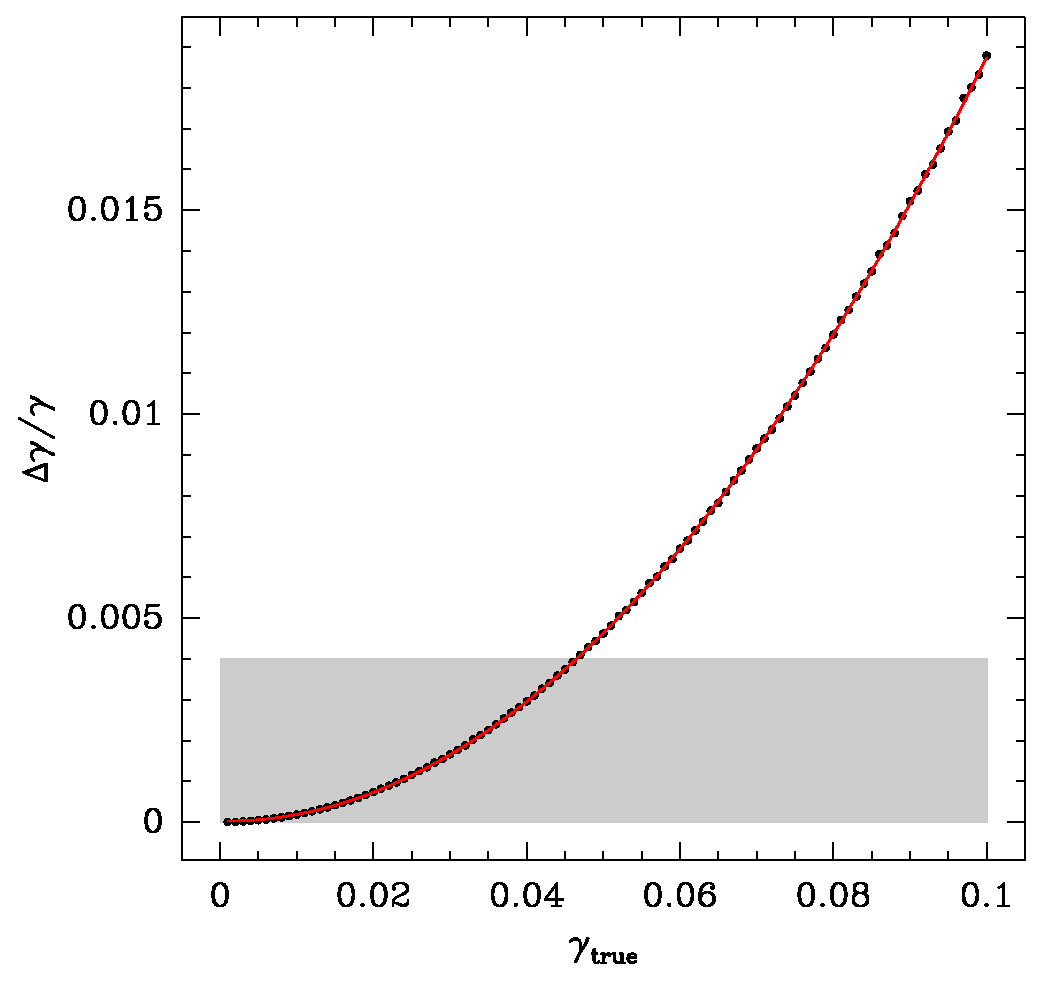
\includegraphics[scale=0.45]{figures/fracerr-vs-shear.eps}
 \caption{Fractional bias in the recovered shear $\Delta g/g = g/g_{true}-1$
     as a function of true shear,
     in a zero noise simulation.  The blue circles represent the recovered
     shear when using the posterior equations expanded to second order about
     zero shear.  The red diamonds represent expansion about the true shear.
     The solid curve represents the best-fitting quadratic function of the true
     shear $\Delta g/g \sim 1.9~g^2_{true}$.  The quadratic bias as a function of
     true shear indicates a break down of the second-order Taylor approximation
 presented in \citet{ba14}. The light and dark gray bands represent the
 approximate requirements for current and planned surveys respectively.}
 \label{fig:nonoise}
\end{figure}

Because of this bias, I expanded the equations about the true shear rather than
zero shear, as explained in \S \ref{sec:impl}.

\subsection{Calibration Bias vs. Galaxy Signal-to-noise Ratio} \label{sec:snbias}

Figure \ref{fig:fracerr} contains the fractional error in the recovered shear
as a function of optimal, matched signal-to-noise ratio \Msn, for the simulated
galaxies described in the previous sections.  For these controlled conditions
this implementation is unbiased at the $\Delta g/g \sim 2\times 10^{-3}$ level.

\begin{figure}
 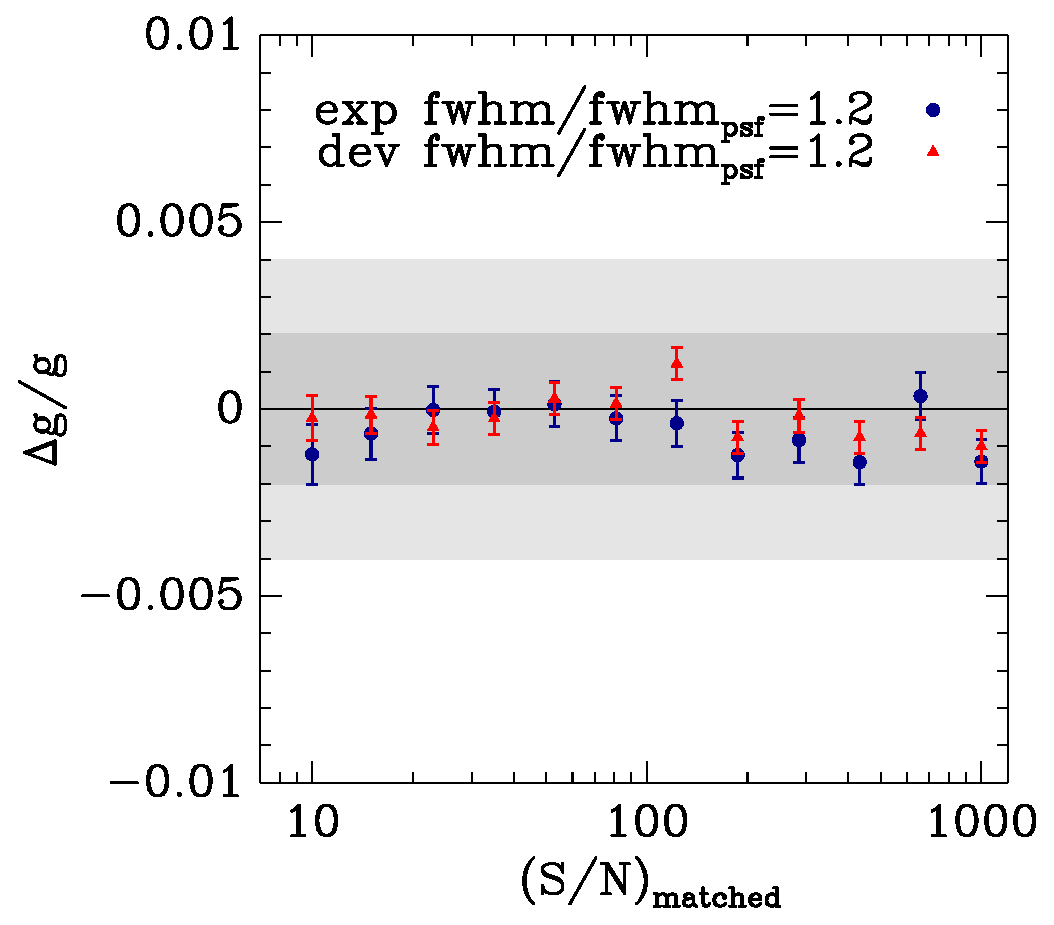
\includegraphics[scale=0.45]{figures/ngmix-fwhm1.2.eps}
 \caption{ Fractional bias in the recovered shear for the estimator presented
     in \citet{ba14}.  The bias is plotted as a function of the maximal, matched
     galaxy signal-to-noise ratio \Msn, for galaxies with exponential (\sersic\
     $n=1$) and \devauc\ profiles ($n=4$).  The simulated galaxy parameters
     were drawn from broad distributions in size, flux, and ellipticity.  The
     size distribution was log-normal with \lognormscatt\% scatter and mean
     such that the {\it observed, post-PSF} FWHM was approximately 1.2 times
     that of the PSF, mimicking the smallest faint galaxy that may pass a size
     cut, such as that used during star-galaxy separation.  The flux
     distribution was log-normal with \lognormscatt\% scatter, and mean chosen
     to produce the indicated signal-to-noise ratio.  The ellipticities were
     drawn from the simple distribution introduced in \citet{ba14}. Under these
     controlled conditions, this shear estimator meets the approximate accuracy
 requirements for current surveys, shown as the light gray band, and the future
 surveys, shown as the dark gray band.}
 \label{fig:fracerr}
\end{figure}

The errors for the different values of \Msn\ appear to be correlated.  This may
be due to the particulars of how the likelihood surface was explored, and may be
correctable by tuning the parameters of the affine-invariant MCMC chain, such
as number of walkers, burn-in, or post-burn-in steps.

\subsection{Comparison with Requirements for Current and Planned Surveys}
\label{sec:req}

In the figures above I showed gray bands representing the approximate
multiplicative bias requirements for current surveys such as the Dark Energy
Survey \citep[][DES]{DESWhitePaper} and the Hyper-Suprime-Cam survey
\citep[][HSC]{HSC12}, and planned surveys such as the Large Synoptic Survey
Telescope survey \citep[][LSST]{IvezicLSST08} and the Euclid Mission
\citep{Euclid2011}.  These requirements are based on the calculations presented
by \citet{HutererSystematics06}, assuming fiducial sky coverage and a
degradation in the dark energy equation of state parameter of less than 20\%.
The cut at 20\% is somewhat arbitrary, and was chosen to coincide very roughly
with the ``official'' requirements for DES. The requirements are $\sim$\desreq\
for current surveys and $\sim$\lsstreq\ for planned surveys.  These
requirements are met in all the cases that I tested.

Smaller and fainter galaxies might have more bias than the average.  The
authors of \cite{ba14} noted that small and faint galaxies, for which the
ellipticity likelihood is broad, get little weight in the average shear
measurement relative to larger and brighter galaxies.  This is an intrinsic
feature of the estimator, no additional weighting is needed.  Indeed I made no
cuts on the simulated galaxies used for this measurement, even though some had
signal-to-noise ratio much less than 10, yet I recovered the shear with good
accuracy.  This is useful, as the shear measurement process need not
necessarily introduce any additional selection effects.

In Figure \ref{fig:nonoise} I showed the multiplicative bias due to the
breakdown of the second-order Taylor expansion at higher shear.   This effect
is prohibitive for current surveys when the shear exceeds 0.05.  The authors of
BA14 suggested potentially using higher order information to tweak the second
order equations.  I have not yet explored that approach.

%One possibility is iteration: in a case where the shear field
%is predicted directly using some functional form, or if it is assumed to be
%constant in some patch of the sky, one might expand about the predicted shear
%field in a second iteration to refine the result; such a method would not
%likely work for cross-correlation lensing, however.  Perhaps a full mapping of
%the posterior of the shear could also be performed, but this would require
%keeping a large amount of information per galaxy.  

\section{Discussion} \label{sec:summary}

But the success of this method in a controlled simulation is a strong
encouragement for further development of this method.  However, the
model-fitting approach I presented here may ultimately only be useful as a
proof-of-principle: model-fitting is limited by the accuracy of the models to
represent true galaxies, and thus in real data additional errors will be
present; this is the so-called ``model bias''.  

\cite{Kacprzak13} showed that model bias may be on the order of baseline
requirements for current surveys, but potentially crippling for future surveys
with more stringent requirements. One potential solution is to fit models with
more freedom.  However, more complex models have more complex likelihood
surfaces, which requires more burn-in for an MCMC chain and more samples to
estimate the expectation values for the $P$, \vecQ\ and \matR\ parameters.
I leave exploration of more complex models to future work.

%In the absence of an absolute calibration source for weak lensing, confidence
%in any technique must ultimately be derived from comparisons with other
%non-lensing measurements and from simulations.  The \texttt{real\_galaxy}
%branch of the Third Gravitational Lensing Accuracy Testing challenge
%\citep[GREAT3,][]{great3} provides an excellent test of shear recovery from
%real galaxy images.  Going forward, such simulation efforts will be of primary
%importance in evaluating the implementation presented here.

As an alternative to model fitting, \cite{ba14} propose to measure moments in
Fourier space, making no explicit parameterization of galaxy light
distributions beyond the observed pixel values, avoiding large model bias.  The
moments are interpreted using a Bayesian formalism similar to that used for model
fitting, and so could be robust to noise bias effects.  Evalutaion of this
Fourier method in the presence of noise is worthy of future effort.

\section*{Acknowledgments}

ES is supported by DOE grant DE-AC02-98CH10886.

Thanks to Gary Bernstein, Bob Armstrong, Jim Bosch, Mike Jarvis and Robert
Lupton for many useful discussions; thanks to An$\check{\textrm{z}}$e Slosar for
suggesting I expand the equations about the true shear to reduce the number of
simulated images required for each test.  Thanks to the STAR, PHENIX and LBNE
experiments at BNL for use of spare cycles on their compute clusters, and to
the RACF staff at BNL for their continued, and disproportionately large support
of my work.


\bibliographystyle{mn2e}
% Bib database
\bibliography{apj-jour,astroref}

\end{document}

